% Group 21 -- PPAI paper presentation (Task II) + Task III progress
% Build: xelatex Group21_PPAI_Presentation.tex   (run twice: overlays use remember picture)
\RequirePackage{fix-cm}
\documentclass[aspectratio=169,10pt]{beamer}
\usepackage{fontspec}
\setsansfont{Liberation Sans}
\setmainfont{Liberation Sans}
\setmonofont{Liberation Mono}
\usefonttheme{professionalfonts}
\usepackage{amsmath,amssymb}
\usepackage{tikz}
\usetikzlibrary{positioning,arrows.meta,calc,fit,backgrounds}
\usepackage{fontawesome5}
\usepackage{pifont}

% ---------- palette (taken from the reference deck) ----------
\definecolor{ppOrange}{HTML}{E69138}
\definecolor{ppOrangeL}{HTML}{FDF1E4}
\definecolor{ppOrangeD}{HTML}{B45F06}
\definecolor{ppBlue}{HTML}{3D85C6}
\definecolor{ppBlueL}{HTML}{E6EFF8}
\definecolor{ppPurple}{HTML}{8E7CC3}
\definecolor{ppPurpleD}{HTML}{674EA7}
\definecolor{ppPurpleL}{HTML}{EFEBF8}
\definecolor{ppGreen}{HTML}{6AA84F}
\definecolor{ppGreenD}{HTML}{38761D}
\definecolor{ppGreenL}{HTML}{EDF6E8}
\definecolor{ppGrey}{HTML}{9E9E9E}
\definecolor{ppText}{HTML}{1A1A1A}
\definecolor{ppMuted}{HTML}{666666}
\definecolor{ppRed}{HTML}{CC0000}

% ---------- type sizes ----------
\newcommand{\fsA}{\fontsize{5.6}{6.8}\selectfont}
\newcommand{\fsB}{\fontsize{6.4}{7.8}\selectfont}
\newcommand{\fsC}{\fontsize{7}{8.5}\selectfont}
\newcommand{\fsD}{\fontsize{8.2}{9.8}\selectfont}
\newcommand{\fsE}{\fontsize{10}{12}\selectfont}
\hyphenpenalty=10000
\exhyphenpenalty=10000

% ---------- frame look ----------
\setbeamertemplate{navigation symbols}{}
\setbeamersize{text margin left=7mm,text margin right=7mm}
\setbeamercolor{normal text}{fg=ppText}
\setbeamercolor{frametitle}{fg=black}
\setbeamerfont{frametitle}{size=\fontsize{14}{16}\selectfont,series=\bfseries}
\setbeamerfont{framesubtitle}{size=\fontsize{7.8}{9.4}\selectfont,series=\mdseries}
\setbeamertemplate{frametitle}{%
  \vspace*{3.4mm}\insertframetitle\par\vspace{1.3mm}%
  {\usebeamerfont{framesubtitle}\color{ppText}\insertframesubtitle}\par}
\setbeamertemplate{footline}{%
  \hspace*{6mm}{\fsA\color{ppGrey}Group 21 \textperiodcentered{} PPAI (IEEE INFOCOM 2026)}\hfill
  {\fsA\color{ppGrey}\insertframenumber}\hspace*{6mm}\vspace*{2.6mm}}

% ---------- helpers ----------
% canvas: absolute layout in cm, origin top-left of the slide, y grows downward
\newenvironment{canvas}%
  {\begin{tikzpicture}[remember picture,overlay,shift={(current page.north west)},x=1cm,y=-1cm]}%
  {\end{tikzpicture}}
\newcommand{\takeaway}[1]{%
  \begin{tikzpicture}[remember picture,overlay]
    \node[anchor=south,text width=14.6cm,align=center,font=\bfseries\fontsize{8.8}{10.6}\selectfont]
      at ([yshift=6.8mm]current page.south) {#1};
  \end{tikzpicture}}
\newcommand{\lab}[1]{{\fsA\color{ppMuted}#1}\\[0.6mm]}
\newcommand{\ttl}[1]{{\fsD\bfseries #1}\\[0.8mm]}
\newcommand{\src}[1]{{\fsA\color{ppMuted}#1}}
\newcommand{\bul}{\textbullet~}
\newcommand{\yes}{{\color{ppGreenD}\faCheck}}

\tikzset{
  panel/.style={draw=ppGrey,line width=0.6pt,rounded corners=2.5mm,fill=white,
    inner sep=2.1mm,align=left,anchor=north west,font=\fsC},
  opanel/.style={panel,draw=ppOrange,fill=ppOrangeL},
  bpanel/.style={panel,draw=ppBlue,fill=ppBlueL},
  ppanel/.style={panel,draw=ppPurple,fill=ppPurpleL},
  gpanel/.style={panel,draw=ppGreen,fill=ppGreenL,dashed},
  chip/.style={rounded corners=1.2mm,inner sep=1.1mm,font=\fsB\bfseries},
  arr/.style={-{Stealth[length=1.8mm]},line width=0.7pt,draw=ppText!80},
  darr/.style={arr,dashed},
  peer/.style={draw=ppGrey,line width=0.6pt,rounded corners=1.5mm,fill=white,
    minimum width=2.2cm,minimum height=0.95cm,align=center,font=\fsB},
  fignote/.style={font=\fsA,text=ppMuted,align=center},
  mini/.style={draw=ppOrange,fill=white,rounded corners=1mm,font=\fsA,minimum width=1.0cm,minimum height=0.42cm},
}

% load bar:  \loadbar{(x,y)}{fraction}{colour}
\newcommand{\loadbar}[3]{%
  \fill[#3] #1 rectangle ++({1.2*#2},0.14);
  \draw[ppGrey,line width=0.4pt] #1 rectangle ++(1.2,0.14);}

% Paper figures, cropped as vectors from the original PDF (viewport in pt, origin bottom-left)
\newcommand{\paper}{figures/paper.pdf}
\newcommand{\figOne}[1]{\includegraphics[page=1,viewport=315 422 563 569,clip,#1]{\paper}}
\newcommand{\figTwo}[1]{\includegraphics[page=3,viewport=50 596 281 749,clip,#1]{\paper}}
\newcommand{\figThree}[1]{\includegraphics[page=3,viewport=79 470 281 551,clip,#1]{\paper}}
\newcommand{\figFour}[1]{\includegraphics[page=3,viewport=306 660 564 742,clip,#1]{\paper}}
\newcommand{\figFive}[1]{\includegraphics[page=4,viewport=311 619 564 742,clip,#1]{\paper}}
\newcommand{\figSix}[1]{\includegraphics[page=5,viewport=77 544 564 742,clip,#1]{\paper}}
\newcommand{\figEight}[1]{\includegraphics[page=9,viewport=70 479 281 542,clip,#1]{\paper}}
\newcommand{\figNine}[1]{\includegraphics[page=9,viewport=310 565 564 747,clip,#1]{\paper}}
\newcommand{\figTen}[1]{\includegraphics[page=9,viewport=310 446 564 531,clip,#1]{\paper}}
\newcommand{\tabOne}[1]{\includegraphics[page=8,viewport=99 583 515 729,clip,#1]{\paper}}

\title{PPAI: Personalized LLM Agent Interoperability}
\author{Group 21: Adele Chinda, Trilok Padhi}

\begin{document}

% =====================================================================
% 1. TITLE
% =====================================================================
\begin{frame}[plain]
\begin{canvas}
  \node[font=\bfseries\fontsize{16.5}{20}\selectfont] at (8,1.2) {PPAI: Personalized LLM Agent Interoperability};
  \node[font=\bfseries\fontsize{10.5}{12.5}\selectfont,text=ppMuted] at (8,1.85) {for Collaborative Edge Intelligence};
  \node[font=\fontsize{8.6}{10.3}\selectfont] at (8,2.5)
    {BitTorrent for expertise: send each question to a peer whose agent knows the answer, and is free.};
  \node[font=\fsB,text=ppMuted] at (8,2.95)
    {Z.~Wang, Q.~Liu, K.~Guo, H.~Wang, J.~Lin, Z.~Hong, S.~Guo \textperiodcentered{} HKUST \& SYSU \textperiodcentered{} IEEE INFOCOM 2026};

  % --- illustration ---
  \node[peer,fill=ppPurpleL,draw=ppPurple,minimum width=2.3cm] (me) at (2.7,5.0)
    {{\fsE\color{ppPurpleD}\faLaptop}\\ your agent: \textbf{law}};
  \node[draw=ppPurple,rounded corners=1.5mm,fill=white,font=\fsA,align=center,text width=2.5cm] at (2.7,3.95)
    {``How are my stock options taxed?''};
  \node[draw=ppOrange,fill=ppOrangeL,line width=0.8pt,rounded corners=2mm,font=\fsC\bfseries,
        align=center,minimum width=2.0cm,minimum height=0.95cm,text=ppOrangeD] (pp) at (6.2,5.0)
    {PPAI\\[-0.4mm]{\fsA\mdseries\color{ppText}score \,+\, route}};
  \draw[arr] (me) -- (pp);

  \node[peer] (p1) at (10.3,3.95) {\faChartLine~ finance agent};
  \node[peer,draw=ppGreen,line width=0.9pt,fill=ppGreenL] (p2) at (10.3,5.1) {\faChartLine~ finance agent};
  \node[peer] (p3) at (10.3,6.25) {\faStethoscope~ medical agent};
  \draw[darr,ppGrey] (pp.east) -- (p1.west);
  \draw[arr,ppGreenD,line width=1pt] (pp.east) -- (p2.west);
  \draw[darr,ppGrey] (pp.east) -- (p3.west);
  \loadbar{(11.7,3.88)}{0.92}{ppRed!75}
  \loadbar{(11.7,5.03)}{0.22}{ppGreen}
  \loadbar{(11.7,6.18)}{0.15}{ppGreen}
  \node[font=\fsA,text=ppMuted,anchor=west] at (11.65,3.62) {load};
  \node[font=\fsA,anchor=west,text=ppRed] at (13.0,3.95) {right skill, busy};
  \node[font=\fsA\bfseries,anchor=west,text=ppGreenD] at (13.0,5.1) {right skill, free \yes};
  \node[font=\fsA,anchor=west,text=ppMuted] at (13.0,6.25) {free, wrong skill};

  \node[font=\fontsize{9}{11}\selectfont] at (8,7.45)
    {\textbf{Group 21} \textperiodcentered{} Adele Chinda (002831349) \textperiodcentered{} Trilok Padhi (002716700)};
  \node[font=\fsB,text=ppMuted] at (8,7.95)
    {CSC 8220 Advanced Computer Networks \textperiodcentered{} Georgia State University \textperiodcentered{} Instructor: Prof.\ Xiaojun Cao \textperiodcentered{} Fall 2026};
\end{canvas}
\end{frame}

% =====================================================================
% 2. BIG PICTURE
% =====================================================================
\begin{frame}
\frametitle{One INFOCOM paper, built from three older ideas}
\framesubtitle{P2P lookup, LLM routing and congestion games meet in PPAI. Our Task III starts where PPAI stops.}
\begin{canvas}
  \node[panel,text width=4.05cm] (t1) at (0.7,1.95)
    {\lab{THREAD 1 \textperiodcentered{} 2002--2005}\ttl{Peer-to-peer networks}
     BitTorrent, Kademlia, gossip: find data among churning peers.};
  \node[panel,text width=4.05cm] (t2) at ([yshift=-1.8mm]t1.south west)
    {\lab{THREAD 2 \textperiodcentered{} 2024--2025}\ttl{LLM routers}
     RouterDC, KABB, RouteLLM: best model per query, on \emph{one} machine.};
  \node[panel,text width=4.05cm] (t3) at ([yshift=-1.8mm]t2.south west)
    {\lab{THREAD 3 \textperiodcentered{} 2002}\ttl{Congestion games}
     Selfish routing costs at most 5/3 of the optimum (Roughgarden \& Tardos).};

  \node[opanel,text width=3.95cm] (pp) at (5.7,2.2)
    {\lab{\color{ppOrangeD}STATE OF THE ART \textperiodcentered{} INFOCOM 2026}\ttl{PPAI}
     Every user runs \textbf{one} specialised LLM agent at the edge. A query the local agent is weak at
     goes to a peer whose agent is strong at it \textbf{and} not overloaded.\\[17mm]
     \mbox{}\hfill{\fsA\color{ppMuted}reported: +7.96 pts, $-$16.34\% time}\hfill\mbox{}};
  \node[mini,draw=ppPurple] (m1) at (6.55,5.3) {query};
  \node[mini] (m2) at (7.9,5.3) {score};
  \node[mini] (m3) at (9.25,5.3) {route};
  \draw[arr] (m1)--(m2); \draw[arr] (m2)--(m3);
  \foreach \t in {t1,t2,t3} \draw[arr] (\t.east) -- (pp.west |- \t.east);

  \node[gpanel,text width=3.7cm] (nx) at (11.4,2.8)
    {\lab{\color{ppGreenD}TASK III \textperiodcentered{} OUR PROJECT}\ttl{Where does it break?}
     PPAI routes on \emph{reported} load. What if the report is old, everyone reacts to it at once, or a peer lies?\\[1.5mm]
     \centering{\fsE\color{ppGreenD}\faClock[regular]\quad\faUsers\quad\faUserSecret}};
  \draw[darr] (pp.east |- nx.west) -- (nx.west);
\end{canvas}
\takeaway{PPAI = P2P lookup for \emph{expertise} + LLM routing + a load-aware game between users.}
\end{frame}

% =====================================================================
% 3. BACKGROUND
% =====================================================================
\begin{frame}
\frametitle{Every laptop can now host a specialist agent, but only one}
\framesubtitle{Small open models plus fine-tuning or RAG make personal agents cheap. Hosting every domain locally is not.}
\begin{canvas}
  \node[anchor=north west] (f1) at (0.6,2.0) {\figOne{width=6.0cm}};
  \node[fignote,anchor=north,text width=6cm] at ([yshift=-1mm]f1.south) {Paper Fig.\ 1: the vision. Each house is one user with one personalised agent.};

  \node[panel,text width=3.75cm] (ag) at (7.0,2.0)
    {\ttl{What is an LLM agent?}
     An LLM plus a \textbf{system prompt}, a \textbf{knowledge base} and \textbf{tools}, which plans and acts toward a goal.
     Personalised by fine-tuning or by its own documents (RAG).};
  \node[panel,text width=3.75cm] (ed) at ([yshift=-2.2mm]ag.south west)
    {\ttl{Why at the edge?}
     Privacy, low latency, no cloud bill: a consumer GPU runs a 7--8B model.
     The catch: it holds \textbf{one} specialist, not five.};

  \node[opanel,text width=3.6cm] (an) at (11.5,2.0)
    {\ttl{The P2P analogy}
     {\fsB\bfseries\color{ppMuted}2003 \textperiodcentered{} BitTorrent}\\
     Missing a piece of a file? Download it from a peer who has it.\\[1.6mm]
     {\fsB\bfseries\color{ppOrangeD}2026 \textperiodcentered{} PPAI}\\
     Your agent is weak at a question? Send it to a peer whose agent is strong at it.\\[1.6mm]
     {\fsB The twist: peers hold \emph{different skills}, not copies of the same file, and a skill can be busy.}};
\end{canvas}
\takeaway{Each user hosts one expert; together, the network hosts all of them.}
\end{frame}

% =====================================================================
% 4. MOTIVATION (Findings 1-3)
% =====================================================================
\begin{frame}
\frametitle{No agent wins everywhere, and the second-best is close}
\framesubtitle{Paper \S III: five 7--8B edge models (Qwen2.5, DeepSeek-R1-Distill, Nemotron-Code, HuatuoGPT-o1, Llama-3) on MMLU.}
\begin{canvas}
  \node[anchor=north] (a) at (2.95,1.95) {\figTwo{width=4.6cm}};
  \node[anchor=center] (b) at (8.0,3.45) {\figThree{width=4.7cm}};
  \node[anchor=center] (c) at (13.05,3.45) {\figFour{width=4.8cm}};
  \node[fignote] at (2.95,5.15) {Fig.\ 2: accuracy per MMLU task};
  \node[fignote] at (8.0,5.15) {Fig.\ 3: how often each agent ranks top-1 / 2 / 3};
  \node[fignote] at (13.05,5.15) {Fig.\ 4: points lost using the 2nd / 3rd best};

  \node[bpanel,text width=4.35cm,minimum height=1.75cm] at (0.7,5.45)
    {\lab{\color{ppBlue}FINDING 1}{\bfseries Agents are specialists.} Agent 4 leads medicine, Agents 1--2 lead maths. Together they cover what none covers alone.};
  \node[ppanel,text width=4.35cm,minimum height=1.75cm] at (5.6,5.45)
    {\lab{\color{ppPurpleD}FINDING 2}{\bfseries A few agents win most tasks.} Always routing to the top-1 piles queries onto Agents 1 and 4: congestion.};
  \node[opanel,text width=4.35cm,minimum height=1.75cm] at (10.5,5.45)
    {\lab{\color{ppOrangeD}FINDING 3}{\bfseries Second-best is nearly as good.} Top-1 $\rightarrow$ top-2 costs $<$5 pts on many tasks, and doubles the candidate pool.};
\end{canvas}
\takeaway{Route to a \emph{good-enough, free} peer, not always to the best one. That is the design in one line.}
\end{frame}

% =====================================================================
% 5. RELATED WORK
% =====================================================================
\begin{frame}
\frametitle{Related work, and the gap PPAI targets}
\framesubtitle{LLM routers assume every model sits on one machine; P2P systems assume every peer holds the same kind of data.}
\newcommand{\full}{\tikz\fill[ppBlue] (0,0) circle (1.1mm);}
\newcommand{\half}{\tikz{\draw[ppBlue,line width=0.6pt] (0,0) circle (1.1mm); \fill[ppBlue] (0,-1.1mm) arc (-90:90:1.1mm) -- cycle;}}
\newcommand{\none}{\tikz\draw[ppBlue,line width=0.6pt] (0,0) circle (1.1mm);}
\begin{canvas}
  \foreach \x/\t in {5.9/{decentralised\\(P2P)}, 7.9/{different skills\\per node}, 9.9/{survives churn\\w/o retraining}, 11.9/{load-aware\\routing}}
    \node[font=\fsB\bfseries,align=center] at (\x,2.35) {\t};
  \foreach \y/\n/\s/\a/\b/\c/\d in {
      3.15/{BitTorrent, Kademlia, gossip}/{2002--2005 \textperiodcentered{} file sharing}/\full/\none/\full/\half,
      3.9/{RouterDC}/{NeurIPS 2024 \textperiodcentered{} trained central router}/\none/\full/\none/\none,
      4.65/{KABB}/{ICML 2025 \textperiodcentered{} knowledge graph of experts}/\none/\full/\half/\none,
      5.4/{RouteLLM and cost-aware routers}/{ICLR 2025 \textperiodcentered{} cost vs.\ quality}/\none/\full/\none/\half}{
    \node[anchor=west,font=\fsC\bfseries] at (0.8,\y-0.1) {\n};
    \node[anchor=west,font=\fsA,text=ppMuted] at (0.8,\y+0.19) {\s};
    \node at (5.9,\y) {\a}; \node at (7.9,\y) {\b}; \node at (9.9,\y) {\c}; \node at (11.9,\y) {\d};
    \draw[ppGrey!50] (0.8,\y+0.37) -- (12.9,\y+0.37);
  }
  \draw[ppOrange,fill=ppOrangeL,line width=0.8pt,rounded corners=2mm] (0.6,5.95) rectangle (13.05,6.75);
  \node[anchor=west,font=\fsD\bfseries,text=ppOrangeD] at (0.8,6.25) {PPAI};
  \node[anchor=west,font=\fsA,text=ppMuted] at (0.8,6.52) {INFOCOM 2026 \textperiodcentered{} this paper};
  \foreach \x in {5.9,7.9,9.9,11.9} \node at (\x,6.35) {\full};
  \node[font=\fsA,text=ppMuted,anchor=west] at (0.8,7.05)
    {filled = designed for it \textperiodcentered{} half = partly \textperiodcentered{} empty = not addressed (as characterised in PPAI \S II)};

  \node[panel,text width=1.85cm,font=\fsA] at (13.3,2.0)
    {{\fsB\bfseries Orthogonal}\\[0.6mm] Quantisation (GPTQ), distillation and pipeline parallelism make each agent cheaper. PPAI can use them unchanged.};
  \node[panel,text width=1.85cm,font=\fsA] at (13.3,4.45)
    {{\fsB\bfseries Agents}\\[0.6mm] Mind2Web, SWE-agent, MetaGPT; on-device: Mobile-Agent-v2, MiniRAG. All single-user.};
\end{canvas}
\takeaway{PPAI claims to be the first to route queries to specialised agents across a churning P2P network.}
\end{frame}

% =====================================================================
% 6. CHALLENGES + OVERVIEW
% =====================================================================
\begin{frame}
\frametitle{Two challenges, two modules}
\framesubtitle{Which peer \emph{can} answer this query? And which peer \emph{should}, when load changes faster than anyone can see?}
\begin{canvas}
  \node[ppanel,text width=4.9cm] (c1) at (0.7,1.95)
    {\lab{\color{ppPurpleD}CHALLENGE 1}\ttl{Diverse agents that churn}
     Each node has different skills; agents join, leave and get updated. A trained central router treats agents as fixed classes, so every change means retraining.\\[0.8mm]
     {\fsB\bfseries\color{ppPurpleD}$\rightarrow$ \S V: query--agent pair scoring}};
  \node[opanel,text width=4.9cm] (c2) at ([yshift=-2mm]c1.south west)
    {\lab{\color{ppOrangeD}CHALLENGE 2}\ttl{Load you cannot see}
     A peer's load is stale by the time you hear it. Agents are interchangeable, so if everyone picks the locally best one, it overloads.\\[0.8mm]
     {\fsB\bfseries\color{ppOrangeD}$\rightarrow$ \S VI: Bayesian game scheduler}};

  \node[anchor=north west] (f5) at (6.85,1.95) {\figFive{width=8.3cm}};
  \node[fignote,anchor=north] at ([yshift=-0.8mm]f5.south) {Paper Fig.\ 5: every peer runs the same PPAI module next to its own agent.};
  \node[chip,fill=ppPurpleL,text=ppPurpleD] at (9.0,6.85) {1. scoring $\rightarrow$ shortlist of capable agents};
  \node[chip,fill=ppOrangeL,text=ppOrangeD] at (13.2,6.85) {2. game $\rightarrow$ pick one, given load};
\end{canvas}
\takeaway{Scoring answers ``who can?''; the game answers ``who should, right now?''}
\end{frame}

% =====================================================================
% 7. MODULE 1: PROTOTYPE-ANCHORED SCORING
% =====================================================================
\begin{frame}
\frametitle{Module 1: queries and agents share one prototype space}
\framesubtitle{$K=20$ learned prototypes act as fixed coordinates, so adding an agent never retrains the router.}
\begin{canvas}
  \node[anchor=north west] (f6) at (0.55,1.95) {\figSix{width=9.6cm}};
  \node[fignote,anchor=north west] at (0.6,5.9) {Paper Fig.\ 6 (QAGate): (a) shared space, (b) training, (c) inference, (d) agent joins / updates / leaves.};

  % toy cosine illustration (baseline at y = 7.35)
  \begin{scope}[shift={(0.9,7.35)}]
    \foreach \i/\h in {0/0.05,1/0.55,2/0.85,3/0.1,4/0.0,5/0.3} \fill[ppPurple] (0.28*\i,0) rectangle ++(0.2,-\h*0.75);
    \foreach \i/\h in {0/0.2,1/0.7,2/0.9,3/0.3,4/0.2,5/0.4} \fill[ppBlue] (2.6+0.28*\i,0) rectangle ++(0.2,-\h*0.75);
    \foreach \i/\h in {0/0.9,1/0.2,2/0.15,3/0.8,4/0.6,5/0.2} \fill[ppBlue!40] (5.2+0.28*\i,0) rectangle ++(0.2,-\h*0.75);
    \draw[ppGrey] (-0.05,0) -- (6.9,0);
    \node[font=\fsA\bfseries,text=ppPurpleD,anchor=west] at (-0.1,0.2) {query $\tilde f(q)$};
    \node[font=\fsA\bfseries,text=ppBlue,anchor=west] at (2.5,0.2) {agent A: $p_A$};
    \node[font=\fsA\bfseries,text=ppBlue!60,anchor=west] at (5.1,0.2) {agent B: $p_B$};
    \node[font=\fsB,anchor=west] at (7.2,-0.5) {$s_A=0.97$ \yes};
    \node[font=\fsB,anchor=west] at (7.2,-0.1) {$s_B=0.29$};
  \end{scope}

  \node[ppanel,text width=4.55cm] (s1) at (10.55,1.95)
    {\lab{\color{ppPurpleD}\ding{172}\; QUERY $\rightarrow$ RELEVANCE VECTOR}
     Sentence encoder + MLP gives $h(q)$; take its cosine to each prototype $\mathbb{C}_k$, sharpen (power $\alpha$), keep the top-$p$, renormalise: $\tilde f(q)\in\mathbb{R}^{K}$.
     Trained with a KL loss against soft cluster labels.};
  \node[bpanel,text width=4.55cm] (s2) at ([yshift=-2mm]s1.south west)
    {\lab{\color{ppBlue}\ding{173}\; AGENT $\rightarrow$ CAPABILITY VECTOR}
     Test agent $j$ on a small question set $Q_k$ for each prototype: $p_j=[\text{acc}_{j,1},\dots,\text{acc}_{j,K}]$.};
  \node[opanel,text width=4.55cm] (s3) at ([yshift=-2mm]s2.south west)
    {\lab{\color{ppOrangeD}\ding{174}\; MATCH, AND HANDLE CHURN}
     Score $s(i,j)=\cos\big(\tilde f(q),\,p_j\big)$.
     Join, update or leave = gossip one $K$-vector with a flag and a timestamp.};
\end{canvas}
\takeaway{An agent joining costs one broadcast of 20 numbers, not a retraining job.}
\end{frame}

% =====================================================================
% 8. MODULE 2: BAYESIAN GAME
% =====================================================================
\begin{frame}
\frametitle{Module 2: a Bayesian game decides who \emph{should} serve}
\framesubtitle{Each user trades relevance against an expected cost of delegation, using a belief about every peer's load.}
\begin{canvas}
  \node[panel,text width=5.85cm] (eq) at (0.7,1.95)
    {\ttl{User $i$'s decision for query $q_i$}
     \begin{tabular}{@{}c@{}}
       $\displaystyle z_i=\arg\max_{j\in E_i}\ \underbrace{s(i,j)}_{\text{relevance}}-\ \beta\,\underbrace{c(i,j)}_{\text{cost of delegation}}$\\[5mm]
       $c(i,j)=\mathbb{E}_{\theta_j\sim b_i}[\rho_j]+t^{\text{infer}}_j+t^{\text{trans}}_{ij}$\\[2mm]
       $\mathbb{E}[\rho_j]=\min\{1,\ \rho_j+\delta(\lambda_j-\mu_j)\},\ \ \rho_j=\lambda_j/\mu_j$\\[2.5mm]
       \parbox{5.8cm}{\raggedright\fsB Each peer has a private type $\theta_j=(\mu_j,\lambda_j)$ (service and arrival rate). User $i$ keeps a belief $b_i(\theta_j)$ and updates it by Bayes' rule when $j$ reports its state $\omega_j$:}\\[3.5mm]
       $b_i^{\text{new}}(\theta_j)\propto P(\omega_j\mid\theta_j)\,b_i(\theta_j)$
     \end{tabular}};

  \node[opanel,text width=3.85cm] (alg) at (6.95,1.95)
    {\ttl{Algorithm 1, per query}
     {\fsB
     \textbf{1}\; score every agent: $s(i,j)$\\[0.5mm]
     \textbf{2}\; shortlist $E_i$: agents with $s(i,j)\ge\theta_s$\\[0.5mm]
     \textbf{3}\; ask each candidate for its load and timings\\[0.5mm]
     \textbf{4}\; update beliefs (Bayes)\\[0.5mm]
     \textbf{5}\; compute $c(i,j)$ and the utility\\[0.5mm]
     \textbf{6}\; delegate to the $\arg\max$; serve locally if it is $i$}};

  % candidate illustration
  \node[font=\fsB\bfseries,anchor=west] at (11.65,2.1) {three candidates};
  \foreach \y/\n/\r/\l/\c in {2.65/A/0.95/0.95/ppRed!75, 3.45/B/0.80/0.25/ppGreen, 4.25/C/0.45/0.10/ppGreen}{
    \node[font=\fsB\bfseries,anchor=west] at (11.65,\y+0.13) {\n};
    \fill[ppPurple] (12.1,\y) rectangle ++({1.7*\r},0.12);
    \fill[\c] (12.1,\y+0.2) rectangle ++({1.7*\l},0.12);
  }
  \draw[ppGreenD,line width=0.9pt,rounded corners=1mm] (11.55,3.3) rectangle (14.0,3.85);
  \node[font=\fsA\bfseries,text=ppGreenD,anchor=west] at (14.05,3.58) {pick};
  \node[font=\fsA,text=ppPurpleD,anchor=west] at (11.65,4.75) {top bar: relevance $s$};
  \node[font=\fsA,text=ppMuted,anchor=west] at (11.65,5.0) {bottom bar: expected load};

  \node[ppanel,text width=7.95cm] at ([yshift=-2.5mm]alg.south west)
    {\ttl{$\beta$ is the one knob}
     {\fsB small $\beta$: chase the most relevant agent (best accuracy, risk of queueing)\\
     large $\beta$: spread queries over less loaded substitutes (lower latency, small accuracy loss)}};
\end{canvas}
\takeaway{The game turns Finding 3 into a rule: give up a little relevance to avoid a long queue.}
\end{frame}

% =====================================================================
% 9. THEORY
% =====================================================================
\begin{frame}
\frametitle{What the paper proves about the game}
\framesubtitle{Six results in \S VI-D. The two that matter most: an equilibrium exists, and its inefficiency is bounded.}
\begin{canvas}
  \node[panel,text width=4.35cm,minimum height=1.45cm] at (0.7,1.95)
    {\lab{LEMMA 1}{\bfseries A best response always exists} and is unique (finite candidate set, fixed tie-break).};
  \node[panel,text width=4.35cm,minimum height=1.45cm] at (5.6,1.95)
    {\lab{LEMMA 2}{\bfseries Utility falls as expected load rises:} $\partial U/\partial\,\mathbb{E}[\rho_j]=-\beta<0$.};
  \node[panel,text width=4.35cm,minimum height=1.45cm] at (10.5,1.95)
    {\lab{THEOREM 3}{\bfseries Beliefs converge} almost surely to the true posterior (Doob's martingale theorem).};

  \node[opanel,text width=4.35cm,minimum height=2.05cm] at (0.7,3.65)
    {\lab{\color{ppOrangeD}THEOREM 1}{\bfseries An equilibrium exists.} With $\Phi(z)=\sum_i U(i,z_i)$ the game is an exact potential game, so a pure Bayesian Nash equilibrium exists; unique under strict concavity and consistent beliefs.};
  \node[opanel,text width=4.35cm,minimum height=2.05cm] at (5.6,3.65)
    {\lab{\color{ppOrangeD}LEMMA 3}{\bfseries Users get there.} Each best-response step strictly increases $\Phi$, so the process stops at an equilibrium in finitely many steps.};
  \node[opanel,text width=4.35cm,minimum height=2.05cm] at (10.5,3.65)
    {\lab{\color{ppOrangeD}THEOREM 2}{\bfseries Selfishness costs at most 5/3.} For affine costs the Bayesian price of anarchy is $\le 5/3$, via Roughgarden--Tardos for congestion games.};

  \begin{scope}[shift={(4.6,6.35)}]
    \node[font=\fsA,anchor=east] at (0,0.07) {social optimum};
    \fill[ppGreen] (0.1,0) rectangle (3.9,0.16);
    \node[font=\fsA,anchor=east] at (0,0.42) {worst equilibrium};
    \fill[ppOrange] (0.1,0.35) rectangle (6.43,0.51);
    \node[font=\fsA,anchor=west] at (6.5,0.42) {$\le 5/3\times$ the optimum};
  \end{scope}
\end{canvas}
\takeaway{Claimed: selfish routing settles, and costs at most 5/3 of the optimum. We revisit this on slide 13.}
\end{frame}

% =====================================================================
% 10. EXPERIMENTAL SETUP
% =====================================================================
\begin{frame}
\frametitle{Setup: five real 7--8B models, up to 1000 peers}
\framesubtitle{Built on vLLM (inference) and libp2p (networking). Every number is the mean of 8 runs.}
\begin{canvas}
  \node[panel,text width=4.6cm] (ag) at (0.7,1.95)
    {\ttl{Five agents}
     {\fsB\renewcommand{\arraystretch}{1.12}%
     \begin{tabular}{@{}l@{\ \ }l@{\ \ }l@{}}
       \textbf{A1} & Qwen2.5-7B-Instruct & {\color{ppMuted}code, maths}\\
       \textbf{A2} & DeepSeek-R1-Distill-7B & {\color{ppMuted}reasoning}\\
       \textbf{A3} & Nemotron-Code-7B & {\color{ppMuted}code}\\
       \textbf{A4} & HuatuoGPT-o1-7B & {\color{ppMuted}medicine}\\
       \textbf{A5} & Llama-3-8B-Instruct & {\color{ppMuted}dialogue}
     \end{tabular}\\[1mm]
     Each also gets ShareGPT conversations as knowledge. Scaled to 50 / 100 / 500 / 1000 peers by copying the 5 models with different knowledge.}};
  \node[panel,text width=4.3cm] (wl) at (5.75,1.95)
    {\ttl{Workloads}
     {\fsB
     MMLU, GSM8K (maths), MedQA (medical), ARC-C (science): 75\% train QAGate, 25\% become user queries.\\[1mm]
     AGIEval (Gaokao, GRE, SAT): held out as \textbf{out-of-distribution}.\\[1mm]
     Poisson arrivals at rate $\lambda$: $\lambda=10$ in the main table, up to 100 queries/s in stress tests.}};
  \node[panel,text width=4.6cm] (sy) at (10.5,1.95)
    {\ttl{System}
     {\fsB
     One Xeon Gold 6226 + RTX A6000 per agent.\\
     Link inside a region: 5 ms, 2 Gbps.\\[1mm]
     QAGate: multilingual MPNet sentence encoder + 2-layer MLP; 20 prototype labels from agglomerative clustering.}};

  \node[opanel,text width=14.35cm] at (0.7,5.62)
    {\ttl{Baselines and metrics}
     {\fsB
     \textbf{Single agent} (A1--A5 alone) \textperiodcentered{} \textbf{Majority voting} (ask all five, vote) \textperiodcentered{}
     \textbf{RouterDC} (trained central router) \textperiodcentered{} \textbf{KABB} (knowledge graph of experts).
     The centralised routers are re-implemented inside the same P2P system.\\[0.8mm]
     Metrics: average \textbf{accuracy} (routing quality) and end-to-end \textbf{process time} per query (queueing + inference).}};
\end{canvas}
\takeaway{Five specialists and one router per peer, compared with routers built for a single machine.}
\end{frame}

% =====================================================================
% 11. RESULT 1: TABLE I
% =====================================================================
\begin{frame}
\frametitle{Result 1: as accurate as the right specialist}
\framesubtitle{Paper Table I ($\lambda=10$), redrawn. Grey = whichever single agent is best on that benchmark (A1, A4 or A5).}
\begin{canvas}
  \node[anchor=north west] (ch) at (0.45,1.9) {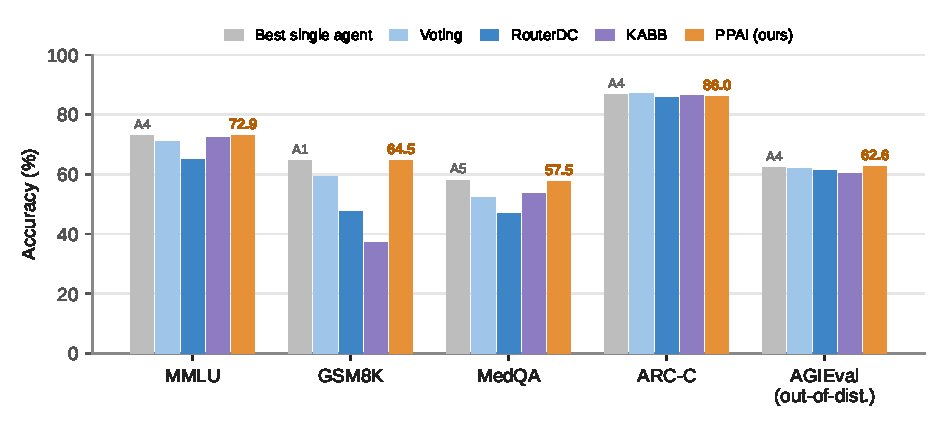
\includegraphics[width=10.3cm]{figures/table1_accuracy.pdf}};
  \node[fignote,anchor=north west] at (0.7,6.6) {Data: paper Table I. Chart: ours. Full table in the backup slide.};

  \node[opanel,text width=3.7cm,align=center] (big) at (11.15,1.95)
    {{\fontsize{20}{22}\selectfont\color{ppOrange}+7.96}\\[0.4mm]
     {\fsB accuracy points on MMLU vs.\ RouterDC (72.94 vs.\ 64.98)}\\[2mm]
     {\fontsize{20}{22}\selectfont\color{ppOrange}$-$16.3\%}\\[0.4mm]
     {\fsB time per query on MMLU vs.\ Voting (21.05 vs.\ 25.16 ms)}};
  \node[panel,text width=3.7cm] at ([yshift=-2.2mm]big.south west)
    {{\fsB Average over the 5 benchmarks: \textbf{68.7\%}. The best \emph{fixed} agent (A1) gets 65.8\%; picking the best agent per benchmark gets 68.9\%.}};
\end{canvas}
\takeaway{PPAI performs as if it knew in advance which specialist to use, without being told.}
\end{frame}

% =====================================================================
% 12. RESULT 2: LOAD AND SCALE
% =====================================================================
\begin{frame}
\frametitle{Result 2: spreading queries keeps latency flat}
\framesubtitle{Stress tests on MMLU. Paper Figs.\ 8--10, cropped from the original PDF.}
\begin{canvas}
  \node[anchor=north west] (f8) at (0.6,1.9) {\figEight{width=6.2cm}};
  \node[font=\fsB,anchor=north west,text width=6.2cm] at ([yshift=-0.5mm]f8.south west)
    {\textbf{Fig.\ 8, arrival rate.} A single agent's time explodes past $\approx$40 queries/s (queueing); PPAI stays lowest up to 50.};
  \node[anchor=north west] (f10) at (0.6,4.6) {\figTen{width=6.2cm}};
  \node[font=\fsB,anchor=north west,text width=6.2cm] at ([yshift=-0.5mm]f10.south west)
    {\textbf{Fig.\ 10, scale} ($\lambda=100$). From 50 to 1000 peers, latency falls 19.6 $\rightarrow$ 17.4 ms; accuracy stays $\approx$73\%.};

  \node[anchor=north west] (f9) at (7.3,1.85) {\figNine{width=5.6cm}};
  \node[opanel,text width=2.0cm,font=\fsB] at (13.15,2.0)
    {\textbf{Fig.\ 9, the $\beta$ knob} ($\lambda=50$)\\[1.2mm]
     $\beta$ from $10^{-5}$ to $10^{-2}$:\\[0.8mm]
     accuracy\\ $\approx$0.72 $\rightarrow$ 0.65\\[0.8mm]
     time\\ $\approx$45 $\rightarrow$ 30 ms\\[0.8mm]
     Bars: usage moves from A1 and A4 to all five agents.};
\end{canvas}
\takeaway{More peers and a larger $\beta$ buy lower latency; accuracy pays only a little.}
\end{frame}

% =====================================================================
% 13. CLOSER LOOK (critique)
% =====================================================================
\begin{frame}
\frametitle{A closer look: what the evidence actually shows}
\framesubtitle{Our own reading, for discussion. The system idea is strong; the evidence for load-awareness is the thinnest part.}
\begin{canvas}
  \node[panel,text width=4.35cm,minimum height=5.1cm] at (0.7,1.95)
    {\lab{1 \textperiodcentered{} RESULTS}\ttl{Headlines are single best-case comparisons}
     \bul ``+7.96\%'' is MMLU vs.\ RouterDC; ``$-$16.34\%'' is MMLU time vs.\ Voting.\\[1mm]
     \bul Against the best single agent on each benchmark, PPAI is
     {\color{ppGreenD}+0.03}, {\color{ppGreenD}+0.01}, {\color{ppRed}$-$0.62}, {\color{ppRed}$-$0.68}, {\color{ppGreenD}+0.49} points.\\[1mm]
     \bul On GSM8K it takes 247 ms; RouterDC takes 103 ms.\\[1.5mm]
     {\fsB\color{ppMuted}The value is \emph{not needing to know} the right agent, not beating it.}};
  \node[opanel,text width=4.35cm,minimum height=5.1cm] at (5.6,1.95)
    {\lab{\color{ppOrangeD}2 \textperiodcentered{} THEORY}\ttl{The proof removes the congestion it is about}
     \bul Theorem 1 uses $\Phi=\sum_i U(i,z_i)$. That is an exact potential only if user $i$'s choice leaves every other user's utility unchanged.\\[1mm]
     \bul And indeed, load enters $U(i,j)$ only through $i$'s \emph{belief}, not through the others' choices: users never interact inside the model.\\[1mm]
     \bul Theorem 2 then borrows the 5/3 bound from congestion games, which needs exactly that interaction.};
  \node[panel,text width=4.35cm,minimum height=5.1cm] at (10.5,1.95)
    {\lab{3 \textperiodcentered{} SYSTEM}\ttl{``Unobservable'' load is polled on every query}
     \bul Algorithm 1 asks every candidate for $(\lambda_j,\mu_j,t^{\text{infer}},t^{\text{trans}})$ on every query: extra round trips that are never measured.\\[1mm]
     \bul The load term is unitless, capped at 1, and added to latencies; $\beta$ had to be swept over $10^{-5}$ to $10^{-2}$.\\[1mm]
     \bul No experiment varies the churn rate or reports gossip and polling traffic.};
\end{canvas}
\takeaway{A clean system idea; how it behaves with stale, shared load information is still open.}
\end{frame}

% =====================================================================
% 14. CONCLUSION
% =====================================================================
\begin{frame}
\frametitle{Conclusion}
\begin{canvas}
  \foreach \y/\n/\h/\b in {
    1.5/1/{Personal edge agents are specialists, so they should share.}/{No agent wins everywhere, a few win most often, and the second-best is usually close (Findings 1--3).},
    3.2/2/{PPAI = prototype-anchored scoring + a Bayesian routing game.}/{Queries and agents share a fixed 20-prototype space, so churn is one gossip message. Each user maximises relevance $-\,\beta\times$ cost of delegation, with an equilibrium and a price of anarchy $\le 5/3$ (as claimed).},
    4.9/3/{It matches the best specialist per benchmark and stays fast under load.}/{Up to +7.96 points vs.\ RouterDC and $-$16.34\% time vs.\ voting on MMLU; flat latency up to 50 queries/s; scales to 1000 peers. Open: stale load, real congestion between users, trust and incentives.}}{
    \draw[ppOrange,line width=0.7pt,rounded corners=2.5mm,fill=white] (0.7,\y) rectangle (15.3,\y+1.45);
    \fill[ppOrange] (1.25,\y+0.48) circle (0.26);
    \node[text=white,font=\fsD\bfseries] at (1.25,\y+0.48) {\n};
    \node[anchor=west,font=\fontsize{9.6}{11.5}\selectfont\bfseries] at (1.7,\y+0.48) {\h};
    \node[anchor=north west,font=\fsB,text width=13.2cm] at (1.7,\y+0.8) {\b};
  }
\end{canvas}
\takeaway{\fontsize{10.5}{12.5}\selectfont Thank you. Next: our Task III progress.}
\end{frame}

% =====================================================================
% 15. TASK III: CANDIDATE PROBLEMS
% =====================================================================
\begin{frame}
\frametitle{Task III progress: three candidate problems}
\framesubtitle{Status: proposal stage. Each is a networking problem with an AI decision-maker, drawn from PPAI's gaps.}
\begin{canvas}
  \draw[ppOrange,line width=0.9pt,dashed,rounded corners=3mm] (0.55,2.15) rectangle (10.15,7.1);
  \node[chip,fill=ppOrange,text=white] at (5.35,2.15) {leading option: A + B together};

  \node[opanel,text width=4.3cm,minimum height=4.5cm] (A) at (0.75,2.45)
    {\lab{\color{ppOrangeD}CANDIDATE A \textperiodcentered{} LOAD BALANCING}
     \ttl{Herding on stale load reports}
     If peers act on old load reports, they all pick the same ``free'' agent at once, overload it, then all leave it
     (Mitzenmacher, \emph{How useful is old information?}).\\[1mm]
     {\bfseries AI:} a (multi-agent) RL policy that decides delegate vs.\ serve locally.\\[1mm]
     {\fsB\color{ppMuted}PPAI's rule is a deterministic argmax, so it is exposed to exactly this.}};
  \node[opanel,text width=4.3cm,minimum height=4.5cm] (B) at (5.55,2.45)
    {\lab{\color{ppOrangeD}CANDIDATE B \textperiodcentered{} CONTROL-PLANE COST}
     \ttl{Probe or guess?}
     Each state request costs a round trip and traffic; skipping it means deciding on a stale belief.
     How many peers should we probe per query, and which?\\[1mm]
     {\bfseries AI:} RL or a bandit that sets the probing budget from the age of each peer's information.\\[1mm]
     {\fsB\color{ppMuted}PPAI polls every candidate on every query and never counts the cost.}};
  \node[panel,text width=4.3cm,minimum height=4.5cm] (C) at (10.6,2.45)
    {\lab{CANDIDATE C \textperiodcentered{} SECURITY}
     \ttl{Trust-aware delegation}
     Malicious peers return wrong answers or flood queries; free-riders consume without serving.
     PPAI \S VII lists both as future work.\\[1mm]
     {\bfseries AI:} Bayesian-bandit reputation plus anomaly detection inside the routing rule.\\[1mm]
     {\fsB\color{ppMuted}Needs a credible attack model to evaluate; the most open-ended option.}};
\end{canvas}
\takeaway{Leading direction: learn \emph{when to delegate and when to probe}, under stale, shared load information.}
\end{frame}

% =====================================================================
% 16. TASK III: DRAFT FORMULATION
% =====================================================================
\begin{frame}
\frametitle{Draft formulation for the leading option}
\framesubtitle{For discussion between us; details will change once we commit to a problem.}
\begin{canvas}
  % diagram
  \node[peer,fill=ppPurpleL,draw=ppPurple,minimum width=2.2cm] (q) at (2.25,2.55) {incoming query $q$\\(task cluster $k$)};
  \node[panel,text width=2.55cm,font=\fsA,anchor=north] (obs) at (2.25,3.45)
    {{\fsB\bfseries observation $o_i$}\\[0.4mm] relevance $\tilde f(q)$ (from PPAI)\\ own queue length\\ last load $\hat\rho_j$ \textbf{and its age} $\Delta_j$ for each candidate};
  \node[draw=ppOrange,fill=ppOrangeL,line width=0.8pt,rounded corners=2mm,align=center,font=\fsC,
        minimum width=2.1cm,minimum height=1.1cm] (pi) at (5.1,3.4) {\textbf{policy} $\pi_\phi$\\{\fsA DQN $\rightarrow$ MAPPO}};
  \draw[arr] (q.east) -- (pi.west);
  \draw[arr] (obs.east) -- (pi.west);
  \node[peer,minimum width=2.15cm] (a1) at (8.0,2.3) {serve locally};
  \node[peer,minimum width=2.15cm] (a2) at (8.0,3.4) {delegate to $j\in E_i$};
  \node[peer,minimum width=2.15cm,draw=ppOrange,line width=0.8pt] (a3) at (8.0,4.5) {probe $m$ peers first};
  \foreach \a in {a1,a2,a3} \draw[arr] (pi.east) -- (\a.west);
  \draw[darr,ppOrange] (a3.south) -- (8.0,5.5) -- node[below,font=\fsA,text=ppOrangeD] {fresh load reports (cost: one RTT each)} (2.25,5.5) -- (obs.south);
  \node[font=\fsA,text=ppMuted,align=center] at (4.9,6.45)
    {environment: discrete-event simulator with one queue per peer,\\ accuracy profiles from PPAI Table I / Fig.\ 2, Poisson + bursty arrivals, churn};

  % right: spec
  \node[opanel,text width=5.5cm] (rw) at (9.6,1.95)
    {\ttl{Reward per query}
     \begin{tabular}{@{}c@{}}
       $r=\text{acc}(j,k)-\beta\,\big(t^{\text{wait}}+t^{\text{infer}}+t^{\text{RTT}}\big)-\gamma\, m$\\[2mm]
       \parbox{5.4cm}{\raggedright\fsB Accuracy of the chosen agent on the query's cluster, minus latency, minus the cost of $m$ probes.}
     \end{tabular}};
  \node[panel,text width=5.5cm] at ([yshift=-2.2mm]rw.south west)
    {{\fsB
     \textbf{Baselines:} PPAI's rule (re-implemented), greedy best-relevance, random among top-3, power-of-two-choices, full-information oracle.\\[1mm]
     \textbf{Metrics:} accuracy, mean and p95 latency, probes per query, Jain's fairness index, behaviour under churn.\\[1mm]
     \textbf{Hypothesis to test:} with stale information PPAI's argmax herds; a learned, partly randomised policy
     lowers p95 latency at equal accuracy and with fewer probes.}};
\end{canvas}
\takeaway{Same inputs as PPAI's router, plus the age of each load report and the option to pay for a fresh one.}
\end{frame}

% =====================================================================
% 17. TASK III: PLAN AND STATUS
% =====================================================================
\begin{frame}
\frametitle{Plan of action and current status}
\framesubtitle{Milestones follow the course schedule. The division of work is tentative until we fix the problem.}
\begin{canvas}
  \draw[ppGrey,line width=1.1pt] (1.0,2.25) -- (15.0,2.25);
  \foreach \x/\c/\t in {3.07/ppGreen/{Now: Task II talk}, 8.07/ppOrange/{Milestone 2: 3-page progress report}, 13.07/ppGrey/{Milestone 3: $\ge$6-page report + 25-min talk}}{
    \fill[\c] (\x,2.25) circle (0.14);
    \node[font=\fsB\bfseries,anchor=south] at (\x,2.02) {\t};
  }
  \node[gpanel,dash pattern=on 0pt off 0pt,text width=4.3cm,font=\fsB,minimum height=2.35cm] at (0.7,2.6)
    {{\fsC\bfseries Done}\\[0.6mm]
     \yes~Read and analysed PPAI in depth\\[0.3mm]
     \yes~Found its gaps: results, proof, overhead\\[0.3mm]
     \yes~Three candidate problems\\[0.3mm]
     \yes~Draft formulation of the leading one};
  \node[opanel,text width=4.3cm,font=\fsB,minimum height=2.35cm] at (5.7,2.6)
    {{\fsC\bfseries Next}\\[0.6mm]
     \bul Choose the problem (A+B or C)\\[0.3mm]
     \bul Build the simulator; re-implement PPAI's rule\\[0.3mm]
     \bul Reproduce herding under stale load reports\\[0.3mm]
     \bul Literature review; IEEE progress report};
  \node[panel,text width=4.3cm,font=\fsB,minimum height=2.35cm] at (10.7,2.6)
    {{\fsC\bfseries Then}\\[0.6mm]
     \bul Train the RL policy (from our Task I DQN)\\[0.3mm]
     \bul Compare with baselines; vary $\beta$, $\gamma$, staleness\\[0.3mm]
     \bul Optional: small vLLM testbed\\[0.3mm]
     \bul Final report and talk};

  \node[panel,text width=6.85cm,font=\fsB] at (0.7,5.25)
    {{\fsC\bfseries Division of work (tentative)}\\[0.6mm]
     \textbf{Adele Chinda:} simulator, RL agent, training\\[0.3mm]
     \textbf{Trilok Padhi:} baselines, workload traces, evaluation and plots\\[0.3mm]
     \textbf{Both:} problem choice, literature review, report, slides};
  \node[ppanel,text width=6.85cm,font=\fsB] at (8.15,5.25)
    {{\fsC\bfseries Open decisions for us}\\[0.6mm]
     \bul Single-agent RL first, or multi-agent from the start?\\[0.3mm]
     \bul Simulation only, or a small real testbed as well?\\[0.3mm]
     \bul Workload: synthetic Poisson, or real LLM traces (Azure, BurstGPT)?};
\end{canvas}
\takeaway{Next two weeks: choose the problem, build the simulator, reproduce PPAI's routing rule.}
\end{frame}

% =====================================================================
% 18. REFERENCES
% =====================================================================
\begin{frame}
\frametitle{References}
\fontsize{6.4}{7.9}\selectfont
\vspace{1mm}
\begin{columns}[T,onlytextwidth]
\begin{column}{0.48\textwidth}
\raggedright
\bul Z.~Wang, Q.~Liu, K.~Guo, H.~Wang, J.~Lin, Z.~Hong, S.~Guo. \textbf{PPAI: Enabling Personalized LLM Agent Interoperability for Collaborative Edge Intelligence.} IEEE INFOCOM 2026. doi:10.1109/INFOCOM59046.2026.11571683.\\[1.1mm]
\bul B.~Cohen. \textbf{Incentives build robustness in BitTorrent.} P2P Econ, 2003.\\[1.1mm]
\bul P.~Maymounkov, D.~Mazi\`eres. \textbf{Kademlia: A peer-to-peer information system based on the XOR metric.} IPTPS, 2002.\\[1.1mm]
\bul M.~Jelasity, A.~Montresor, O.~Babaoglu. \textbf{Gossip-based aggregation in large dynamic networks.} ACM TOCS, 2005.\\[1.1mm]
\bul S.~Chen et al. \textbf{RouterDC: Query-based router by dual contrastive learning for assembling LLMs.} NeurIPS 2024.\\[1.1mm]
\bul J.~Zhang et al. \textbf{KABB: Knowledge-aware Bayesian bandits for dynamic expert coordination in multi-agent systems.} ICML 2025.\\[1.1mm]
\bul I.~Ong et al. \textbf{RouteLLM: Learning to route LLMs from preference data.} ICLR 2025.\\[1.1mm]
\bul J.~Snell, K.~Swersky, R.~Zemel. \textbf{Prototypical networks for few-shot learning.} NeurIPS 2017.
\end{column}
\begin{column}{0.48\textwidth}
\raggedright
\bul T.~Roughgarden, \'E.~Tardos. \textbf{How bad is selfish routing?} Journal of the ACM, 2002.\\[1.1mm]
\bul J.~Li et al. \textbf{More agents is all you need.} TMLR 2024.\\[1.1mm]
\bul M.~Mitzenmacher. \textbf{How useful is old information?} IEEE TPDS, 2000.\\[1.1mm]
\bul M.~Mitzenmacher. \textbf{The power of two choices in randomized load balancing.} IEEE TPDS, 2001.\\[1.1mm]
\bul S.~Kaul, R.~Yates, M.~Gruteser. \textbf{Real-time status: How often should one update?} IEEE INFOCOM 2012.\\[1.1mm]
\bul S.~Kamvar, M.~Schlosser, H.~Garcia-Molina. \textbf{The EigenTrust algorithm for reputation management in P2P networks.} WWW 2003.\\[1.1mm]
\bul V.~Mnih et al. \textbf{Human-level control through deep reinforcement learning.} Nature, 2015.\\[1.1mm]
\bul C.~Yu et al. \textbf{The surprising effectiveness of PPO in cooperative multi-agent games.} NeurIPS 2022 (Datasets \& Benchmarks).
\end{column}
\end{columns}
\end{frame}

% =====================================================================
% 19. BACKUP: TABLE I
% =====================================================================
\begin{frame}
\frametitle{Backup: Table I as printed in the paper}
\framesubtitle{Accuracy (\%) and process time (ms) per query, arrival rate $\lambda=10$.}
\begin{canvas}
  \node[anchor=north] at (8,2.0) {\tabOne{width=13.2cm}};
\end{canvas}
\takeaway{PPAI is best or within about 1 point of the best on every benchmark, and never the slowest multi-agent method.}
\end{frame}

\end{document}
